\documentclass[11pt,aspectratio=169,t]{beamer}
\usepackage{amsmath}
\usetheme[numbering=fraction]{metropolis}
\usepackage[T1]{fontenc}
\usepackage[default]{lato}
%\usepackage{mathpazo}
\usepackage{fourier}
% \usepackage{lmodern}
%\usepackage{concmath}
\usepackage{textcomp}
\usepackage{mathtools}
%\usepackage{skmath}
\usefonttheme{professionalfonts}
\usefonttheme[onlymath]{serif}

\overfullrule=2cm

\setbeamertemplate{footline}{%
  \begin{beamercolorbox}[wd=\textwidth, sep=1ex]{footline}%
    \usebeamerfont{page number in head/foot}%
    \usebeamertemplate*{frame footer}
    \hfill%
    \usebeamertemplate*{frame numbering}
    \quad% 
  \end{beamercolorbox}%
}

%\includeonlyframes{current}

\graphicspath{{assets/}}

\usepackage{algorithm2e}
\usepackage{siunitx}

% Table packages.
\usepackage{booktabs}

\usepackage{xparse}
\usepackage{makecell}
\usepackage{tikz}
\usepackage[beamer,customcolors]{hf-tikz}
\usetikzlibrary{calc}
\usetikzlibrary{decorations.pathreplacing}
\usetikzlibrary{fadings}


\pdfstringdefDisableCommands{%
  \def\\{}%
  \def\texttt#1{<#1>}%
}

% ------------------------------------------------------------------------------
% Define useful colors.
\colorlet{black}{black!50!gray}
\colorlet{green}{green!50!gray}
\colorlet{blue}{blue!50!gray}

\colorlet{CBlue}{blue!15}
\colorlet{CBlueD}{blue!95!gray}
\colorlet{CRed}{red!15}
\colorlet{CRedD}{red!65!gray}
\colorlet{CGreenD}{green!60!gray}
\colorlet{COrange}{orange}

% Background color.
\definecolor{CBackground}{RGB}{255,253,253}
\setbeamercolor{background canvas}{fg=black,bg=CBackground}
% ------------------------------------------------------------------------------

% ------------------------------------------------------------------------------
% tikz settings
\tikzset{   
    every path/.style={thick},
}
% ------------------------------------------------------------------------------

% \usepackage[protrusion,expansion,kerning,spacing,final]{microtype}
% \microtypecontext{spacing=nonfrench}

% ------------------------------------------------------------------------------
% Useful mathematical macros
\newcommand{\Data}{\vec{D}}
\newcommand{\DataExt}{\widetilde{\vec{D}}}
\newcommand{\MSE}{\ensuremath{\text{MSE}}}
\newcommand{\T}{\ensuremath{\text{T}}}
\renewcommand{\vec}[1]{\boldsymbol{#1}}
\newcommand{\VTheta}{\ensuremath{\vec{\theta}}}
\newcommand{\VLambda}{\ensuremath{\vec{\lambda}}}
%\DeclareMathOperator*{\argmin}{arg\,min}
\newcommand{\R}{\mathbb R}
\newcommand{\UNN}[1][\text{NN}]{u_{#1}}
\newcommand{\FNN}[1][\text{NN}]{f_{#1}}
\newcommand{\NonlinOp}{\mathcal N\!}
\newcommand{\Loss}{\mathcal L}
\newcommand{\Model}{\mathcal G}
\newcommand{\ModelT}{\mathrm G}  % Total model: concatenation over dataset.
\newcommand{\given}{|}
\newcommand{\ParamSpace}{\mathcal U}
\DeclarePairedDelimiter\norm{\lVert}{\rVert}
\newcommand{\dd}{\,\textrm{d}}
\renewcommand{\Pr}{\mathbb P}
\renewcommand{\hat}{\widehat}
\newcommand{\upot}{\vec u_{\text{pot}}}
\newcommand{\usol}{\vec u_{\text{sol}}}
\newcommand{\Grad}{\nabla}
\newcommand{\Div}{\nabla \cdot}
\newcommand{\Curl}{\nabla \! \times \!}

\newcommand{\xx}{\vec{x}}

\newcommand{\explain}[2]{\underset{\mathclap{\overset{\uparrow}{#2}}}{#1}}
\newcommand{\explainup}[2]{\overset{\mathclap{\underset{\downarrow}{#2}}}{#1}}

% Useful mathematical macros (end)
% ------------------------------------------------------------------------------

\title{Physics-informed neural networks for discrete Helmholtz--Hodge decomposition}
\author{Dmitry I.\ Kabanov (formerly at RWTH)\\
  Joint work with Luis Espath (U Nottingham), Ra\'ul Tempone (RWTH, KAUST)}
\institute{}
\date{WIAS Berlin, 12 May 2022}
\def\titlepage{%
  \usebeamertemplate{title page}%<---
}
\titlegraphic{\vspace{5.2cm}\hspace{6.3cm}\includegraphics{rwth-logo}\phantom{text}\par}

% ------------------------------------------------------------------------------

\begin{document}

\begin{frame}
\titlepage
\end{frame}

% ------------------------------------------------------------------------------
\begin{frame}{Biography sketch}
\begin{itemize}
    \item 2004–2010: Moscow Engineering-Physics Institute, BSc. + MSc.
    \item 2010—2012: Software developer, Moscow
    \item 2012—2018: King Abdullah University of Science and Technology,
          Saudi Arabia \\
          PhD thesis ``Numerical computation of detonation stability''
          (analysis of stability of traveling-wave solutions of reactive
          Euler equations for compressible fluids via numerical simulation
          and postprocessing)
    \item 2018—2019: Software developer in One Omega Seismics, Saudi Arabia
    \item 2019—March 2022: Postdoc in RWTH Aachen University, Germany\\
          Projects on physics-informed neural networks
\end{itemize}
\end{frame}

\section{Helmholtz--Hodge decomposition}

% ------------------------------------------------------------------------------
\begin{frame}{Introduction}
In 1858 Helmholtz postulated that a vector field $\vec u: \R^{n} \to \R^{n}$
can be decomposed in two subfields:
$$
\vec u = \upot + \usol = \Grad \phi + \Curl \vec\psi
$$
where
\begin{itemize}
  \item $\upot := \Grad \phi$ potential (curl-free) subfield
       % , $\phi: \R^{n}\to\R$
  \item $\usol := \Curl \vec\psi$ solenoidal (divergence-free) subfield
        %, $\vec\psi: \R^{n}\to \R^{n}$
\end{itemize}

\onslide<2->{%
Vector calculus identities clarify the names ``curl-free'' and ``divergence-free'':
$$
\Curl \Grad \phi = 0 \quad \text{ for any } \phi
$$
and
$$
\Div \Curl \vec \psi = 0 \quad \text{ for any } \vec \psi
$$
}
\onslide<3->{%
Nowadays it is called Helmholtz--Hodge decomposition (HHD).
}

\end{frame}
% ------------------------------------------------------------------------------
\begin{frame}{HHD, in general, is not unique}
If $\vec u$ is smooth, then by taking divergence, we find that
$$
\Delta \phi = \Div \vec u
$$
and
$$
\usol = \vec u - \Grad \phi.
$$

However, the decomposition is not unique. For any harmonic function $\xi$
(i.e. $\Delta \xi = 0$),
$$
\vec u = \Grad (\phi + \xi) + \left( \Curl \vec \psi - \Grad \xi \right)
$$
is also a decomposition.

If domain $D=\R^{n}$ and $\vec u$ vanishes as $|\vec x| \to \infty$, then
$\xi \equiv 0$, and the decomposition is unique.

\end{frame}

% ------------------------------------------------------------------------------
\begin{frame}{Orthogonal HHD}
Another way to achieve uniqueness is to impose additional constraints.

For example orthogonality of the subfields in $L^{2}$-sense
\[
\int_{D} \upot \usol \, \dd \vec x = 0
\]
Orthogonality can be achieved by imposing boundary conditions on the flow.
\end{frame}

% ------------------------------------------------------------------------------
\begin{frame}{Orthogonality of subfields}

\emph{Theorem [ChorinMardsen2000]}.
A~vector field $\vec u$ on $D$ can be decomposed
in the form
\[
\vec u = \upot + \usol = \Grad \phi + \usol
\]
with $\Div \usol = 0$.
If $\usol \cdot \vec n = 0$ on $\partial D$, then
$
\int_{D} \upot \usol \, \dd \vec x = 0.
$

\onslide<2->{%
\emph{Proof}.
\begin{align*}
  \Div \left(\phi \usol \right)
  &= \phi \Div \usol + \usol \cdot \Grad \phi && \text{divergence of product} \\
  &= \usol \cdot \Grad \phi && \Div \usol = 0
\end{align*}
}
\onslide<3->{%
\begin{align*}
  \int_{D} \usol \cdot \Grad \phi \, \dd \vec x
  &= \int_{D} \Div \left(\phi \usol\right) \, \dd \vec x && \text{by the above} \\
  &= \oint_{\partial D} \phi \usol \cdot \vec n \, \dd S && \text{Gauss--Ostrogradsky thm}\\
  &= 0 && \usol \cdot \vec n = 0 \text{ on } \partial D
\end{align*}
}

\end{frame}

% ------------------------------------------------------------------------------
\begin{frame}{Uniqueness of orthogonal HHD}
\emph{Theorem. Uniqueness of orthogonal HHD [ChorinMardsen2000]}.
A~vector field $\vec u$ on $D$ can be decomposed
in the form
\[
\vec u = \upot + \usol = \Grad \phi + \usol
\]
with $\Div \usol = 0$.
If $\usol \cdot \vec n = 0$ on $\partial D$, then the decomposition is unique.

Proof.
Let
$$
\vec u = \upot + \usol = \Grad \phi + \usol =
    \Grad \phi' + \usol' = \upot' + \usol'
$$
Both decompositions must be orthogonal
$$
\int_D \Grad \phi \cdot \usol \, \dd \xx = 0 \text{ and }
\int_D \Grad \phi' \cdot \usol' \, \dd \xx = 0.
$$
\end{frame}

%-------------------------------------------------------------------------------
\begin{frame}{Uniqueness of orthogonal HHD}
\emph{Proof (continuation).}
Having
$
\vec u = \Grad \phi + \usol =
    \Grad \phi' + \usol'
$
implies
$$
0 = \Grad \left(\phi - \phi'\right) + \usol - \usol'
$$
and by taking the inner product with $\usol - \usol'$ over $D$, we get
\begin{align*}
0 &= - \int_D \Grad \phi \cdot \usol' + \Grad \phi' \cdot \usol +
    \norm{\usol - \usol'}{}^2 \,\dd \xx \\
  &= - \int_D \Div \left(\phi \usol'\right) + \Div \left(\phi' \usol\right) +
    \norm{\usol - \usol'}{}^2 \,\dd \xx && \Div \usol = \Div \usol' = 0\\
  &= - \oint_{\partial D} \phi \usol' \cdot \vec n
     + \phi' \usol \cdot \vec n \,\dd s
     + \int_D \norm{\usol - \usol'}{}^2 \,\dd \xx && \text{Gauss--Ostrogradsky thm}\\
  &= \phantom{-}\int_D \norm{\usol - \usol'}{}^2 \,\dd \xx,
\end{align*}
which implies that $\usol = \usol'$, and hence, $\Grad \phi = \Grad \phi'$.
\end{frame}

% ------------------------------------------------------------------------------
\section{Discrete Helmholtz--Hodge decomposition}

% ------------------------------------------------------------------------------
\begin{frame}{Discrete Helmholtz--Hodge decomposition}

\begin{minipage}{0.78\textwidth}
Consider a problem in which vector field $\vec u$ is not given analytically
but only as a finite dataset $\mathrm D = (\xx_{i}, \vec u_{i})$ for $i=1,\dots, N$ inside
a~given compact domain $D$.

In this case, we aim to learn the appropriate decomposition via empirical
risk minimization with additional regularizing terms
\[
\phi^{*}, \psi^{*} =
\arg \min_{\phi, \psi} \mathcal L(\phi, \vec \psi, \mathrm D)
\]
where
\[
\mathcal L(\phi, \vec \psi, \mathrm{D}) =
\frac1N \sum_{i=1}^{N} \norm{\Grad \phi(\xx) + \Curl{\vec \psi(\xx)} - \vec u}^{2}_{2}
\]
\end{minipage}
\hfill
\begin{minipage}{0.20\textwidth}
  \centering
  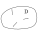
\includegraphics[scale=0.7]{measurements}
\end{minipage}
\end{frame}

% ------------------------------------------------------------------------------
\begin{frame}{Discrete Helmholtz--Hodge decomposition with regularizers}
Using the above results on the uniqueness of the orthogonal HHD, we solve
in~practice the following inverse problem with additional regularizers
\[
\phi^{*}, \psi^{*} =
\arg \min_{\phi, \psi} \mathcal L(\phi, \vec \psi, \mathrm D)
  + \lambda R_{\perp}(\phi, \vec \psi) + \mu R_{\text S}(\phi, \vec \psi)
\]
where
\begin{align*}
&\text{orthogonality regularizer }
&R_{\perp}(\phi, \vec \psi) &=
    \int_{D} \left(\Grad \phi \cdot \Curl \vec \psi \right)^{2} \, \dd \xx \\
&\text{smoothness regularizer }
&R_{\text S}(\phi, \vec \psi) &=
    \int_{D} \norm{\partial^{3}\phi(\xx)}^{2} + \norm{\partial^{3}\vec \psi(\xx)}^{2} \, \dd \xx
\end{align*}

Integral in regularizers are discretized on a uniform grid.

Hyperparameters $\lambda$ and $\mu$ should be set before the training.
We use $\mu=1e-2$ in all experiments but we vary $\lambda$ to study its effect
on the reconstruction performance.

\end{frame}

\begin{frame}{Specialization to 2D}
We consider only two-dimensional case $D \subset \R^{2}$.

Then the vector potential $\vec \psi$ is a vector that is orthogonal to $D$:
\[
 \vec \psi = (0, 0, \psi)
\]
and the curl operator becomes
\[
\Curl \vec \psi = \partial_{2} \psi \vec e_{1} - \partial_{1} \psi \vec e_{2}
\]
where $(\vec e_{1}, \vec e_{2})$ is the canonical basis in $\R^{2}$.

Function $\psi$ is known as \emph{stream function} in fluid mechanics.

Note that 2D decomposition is now defined by two scalar-valued functions $\phi$
and $\psi$.
\end{frame}


% ------------------------------------------------------------------------------
\begin{frame}
\frametitle{Multilayer perceptron neural networks}

As estimating functions $\phi$ and $\psi$ we use two
multilayer perceptrons networks that map \(\R^{2}\) to \(\R\):
\[
    \phi(\xx; \VTheta) = A \circ F_{L} \circ \dots \circ F_1(\xx)
\]
where
\begin{itemize}
    \item \(A\) is linear operator, which is also called \textbf{output layer}
    \item \(F_j : \R^{n_{j-1}} \to \R^{n_j} \) nonlinear continuous
    functions, with \(n_0 = 2\), which are called \textbf{hidden layers},
    of type $\tanh(W_j \, z_{j-1} + b_j)$, where $\tanh$ is applied
    componentwise
    \item \(W_j \in \R^{n_{j-1}} \times \R^{n_j}\) are \textbf{weights} matrices
    \item \(b_j \in \R^{n_j}\) are \textbf{bias} vectors
    \item nonlinear function \(\tanh\) is applied componentwise
\end{itemize}
Parameter vector $\VTheta$ is a concatenation of $A$, $W_{j}$ and $b_{j}$ for
$j = 1, \dots, L$.
\end{frame}

% \begin{frame}{Neural networks - hidden layers}

% We specialize hidden layers $F_{j}$ of a neural network
% \[
%     \phi(\xx; \VTheta) = A \circ F_{L} \circ \dots \circ F_1(\xx)
% \]
% to pairs "nonlinearity + affine map":
% \[
%     F_j(z_{j}) = \sigma(W_j \, z_{j-1} + b_j)
% \]
% where
% \begin{itemize}
%     \item \(W_j \in \R^{n_{j-1}} \times \R^{n_j}\) are \textbf{weights} matrices
%     \item \(b_j \in \R^{n_j}\) are \textbf{bias} vectors
%     \item nonlinear function \(\sigma\) is applied componentwise
% \end{itemize}

% Parameter vector $\VTheta$ is a concatenation of $A$, $W_{j}$ and $b_{j}$ for
% $j = 1, \dots, L$.

% \end{frame}

\begin{frame}
\frametitle{Visualization of multilayer perceptron $\R^2 \to \R$ with one hidden layer}

\begin{figure}[t]
    \centering
    \def\layersep{2.5cm}

    \begin{tikzpicture}[shorten >=1pt,->,draw=black!50, node distance=\layersep]
        \tikzstyle{every pin edge}=[<-,shorten <=1pt]
        \tikzstyle{neuron}=[circle,fill=black!25,minimum size=17pt,inner sep=0pt]
        \tikzstyle{input neuron}=[neuron, fill=CGreenD];
        \tikzstyle{output neuron}=[neuron, fill=CRedD];
        \tikzstyle{hidden neuron}=[neuron, fill=CBlueD];
        \tikzstyle{annot} = [text width=4em, text centered]
    
        % Draw the input layer nodes
        \foreach \name / \y in {1,...,2}
        % This is the same as writing \foreach \name / \y in {1/1,2/2,3/3,4/4}
            \node[input neuron, pin=left:Input \#\y] (I-\name) at (0,-1-\y) {};
    
        % Draw the hidden layer nodes
        \foreach \name / \y in {1,...,5}
            \path[yshift=0.5cm]
                node[hidden neuron] (H-\name) at (\layersep,-\y cm) {};
    
        % Draw the output layer node
        \node[output neuron,pin={[pin edge={->}]right:Output}, right of=H-3] (O) {};
    
        % Connect every node in the input layer with every node in the
        % hidden layer.
        \foreach \source in {1,...,2}
            \foreach \dest in {1,...,5}
                \path (I-\source) edge (H-\dest);
    
        % Connect every node in the hidden layer with the output layer
        \foreach \source in {1,...,5}
            \path (H-\source) edge (O);
    
        % Annotate the layers
        \node[annot,above of=H-1, node distance=1cm] (hl) {Hidden layer};
        \node[annot,left of=hl] {Input layer};
        \node[annot,right of=hl] {Output layer};
    \end{tikzpicture}
\end{figure}

\begin{minipage}{\linewidth}
\centering
\tiny[\url{https://texample.net/tikz/examples/neural-network/}, with modifications]
\end{minipage}
\end{frame}
% ------------------------------------------------------------------------------

% ------------------------------------------------------------------------------
\begin{frame}{Training process and algorithms}

With the above choices for parameterized estimators $\phi(\cdot; \VTheta_{\phi})$
and $\psi(\cdot; \VTheta_{\psi})$, training process amounts to solving the following
optimization problem:
\[
\VTheta_{\phi}^{*}, \VTheta_{\psi}^{*} =
\arg \min_{\VTheta_\phi, \VTheta_\psi} \mathcal L(\phi, \vec \psi, \mathrm D)
  + \lambda R_{\perp}(\phi, \vec \psi) + \mu R_{\text S}(\phi, \vec \psi)
\]

\begin{itemize}
    \item We use ADAM optimizer with default parameters
    \item We initialize parameters using Xavier Glorot initialization
    \item We set initial learning rate to 0.1 to help generalization
    \item We note that decreasing the learning rate after some number
        of iterations helps with training stability and generalization
\end{itemize}
\end{frame}

% ------------------------------------------------------------------------------
\begin{frame}{Generalization error}

We score quality of reconstruction using relative Root Mean Squared Error rRMSE
\[
\text{rRMSE} = \sqrt{%
    \frac{%
    \sum_{i=1}^N \norm{\vec u_i - \hat{\vec u}_i}_2^2}{%
    \sum_{i=1}^N \norm{\vec u_i}2^2
    }
}
\]
where
\begin{itemize}
    \item $\vec u_{i}$ is the $i$th measurement from the test dataset
    \item $\hat{\vec u}_{i}$ the corresponding prediction
\end{itemize}

Measurements are either from total vector field
or from potential or solenoidal subfields.
\end{frame}

\section{Example: Orthogonal decomposition of~a~field with~vanishing normal solenoidal subfield on~the~boundary}

% ------------------------------------------------------------------------------
\begin{frame}{Data}
We consider a vector field given by the following potential
functions:
\begin{align}
\phi &= \exp\left( - \frac{\norm{\vec x - \vec x_0}{}^2}{2} \right)
    - \exp\left( - \frac{\norm{\vec x - \vec x_1}{}^2}{2} \right) \\
\psi &= \exp\left( - \frac{\norm{\vec x - \vec x_2}{}^2}{2} \right),
\end{align}
where $\vec x_0 = (3, -3)$, $\vec x_1 = (-3, -3)$, $\vec x_2 = (0, 3)$.
All points $\vec x$ belong to domain $[-6, 6]^2$.
The vector fields are given by $\Grad \phi$ and $\Curl \psi$, respectively.

Training data are given by uniform grid $51 \times 51$, validation data
by grid $16 \times 16$, test data by grid $101 \times 101$.
\end{frame}

\begin{frame}{Example}
We use a neural network with one hidden layer with 64 hidden neurons.
We train it using \num{100000} epochs.

We analyze the reconstruction performance different values of the multiplier
of the orthogonalization regularizer
$\lambda \in \{  10^{-8}, 10^{-3}, 10^{-2}, 10^{-1}, 1, 10 \}$.
\end{frame}

% ------------------------------------------------------------------------------
\begin{frame}{Example}
\centering
Reconstruction relative mean squared errors $\times 100\%$ versus multiplier of the
orthogonalization regularizer $\lambda$.
Errors $e_{\text{tot}}$, $e_{\text{pot}}$, $e_{\text{sol}}$ are for total field
and potential and solenoidal subfields, respectively.

\centering
\begin{tabular}{lrrrr}
\toprule
{} &   $\lambda$ & $e_{\text{tot}}$ & $e_{\text{pot}}$ & $e_{\text{sol}}$ \\
\midrule
1 & \num{0e+00} &                1 &               95 &              135 \\
2 & \num{1e-03} &                0 &               21 &               29 \\
3 & \num{1e-01} &                0 &                4 &                6 \\
4 & \num{1e+00} &                0 &                2 &                3 \\
5 & \num{1e+01} &                1 &                2 &                4 \\
6 & \num{1e+02} &                1 &                1 &                2 \\
\bottomrule
\end{tabular}

\end{frame}

\begin{frame}{Reconstruction of total field}
\centering
\vspace{0.5cm}
\includegraphics[scale=0.45]{ribeiro/recon-total-first-best}
\begin{tikzpicture}[remember picture, overlay]
\tikzset{shift={(current page.center)}, xshift=-4.3cm, yshift=2cm}
\node (txt) at (0, 0) {True};
\end{tikzpicture}
\begin{tikzpicture}[remember picture, overlay]
\tikzset{shift={(current page.center)}, xshift=0cm, yshift=2cm}
\node (txt) at (0, 0) {$\lambda = 0$};
\end{tikzpicture}
\begin{tikzpicture}[remember picture, overlay]
\tikzset{shift={(current page.center)}, xshift=4.5cm, yshift=2cm}
\node (txt) at (0, 0) {$\lambda = 100$};
\end{tikzpicture}
\end{frame}

\begin{frame}{Reconstruction of potential subfield}
\centering
\vspace{0.5cm}
\includegraphics[scale=0.45]{ribeiro/recon-pot-first-best}
\begin{tikzpicture}[remember picture, overlay]
\tikzset{shift={(current page.center)}, xshift=-4.3cm, yshift=2cm}
\node (txt) at (0, 0) {True};
\end{tikzpicture}
\begin{tikzpicture}[remember picture, overlay]
\tikzset{shift={(current page.center)}, xshift=0cm, yshift=2cm}
\node (txt) at (0, 0) {$\lambda = 0$};
\end{tikzpicture}
\begin{tikzpicture}[remember picture, overlay]
\tikzset{shift={(current page.center)}, xshift=4.5cm, yshift=2cm}
\node (txt) at (0, 0) {$\lambda = 100$};
\end{tikzpicture}
\end{frame}

\begin{frame}{Reconstruction of solenoidal subfield}
\centering
\vspace{0.5cm}
\includegraphics[scale=0.45]{ribeiro/recon-sol-first-best}
\begin{tikzpicture}[remember picture, overlay]
\tikzset{shift={(current page.center)}, xshift=-4.3cm, yshift=2cm}
\node (txt) at (0, 0) {True};
\end{tikzpicture}
\begin{tikzpicture}[remember picture, overlay]
\tikzset{shift={(current page.center)}, xshift=0cm, yshift=2cm}
\node (txt) at (0, 0) {$\lambda = 0$};
\end{tikzpicture}
\begin{tikzpicture}[remember picture, overlay]
\tikzset{shift={(current page.center)}, xshift=4.5cm, yshift=2cm}
\node (txt) at (0, 0) {$\lambda = 100$};
\end{tikzpicture}
\end{frame}

% % ------------------------------------------------------------------------------
% \section{Example 2: Orthogonal decomposition without vanishing normal
% solenoidal subfield on~the~boundary}

% \begin{frame}{Ex 2: Data}
% Potential (curl-free) part given by the subfield:
% \[
%     \upot = \frac12 \left(
%         \begin{array}{r}
%         -2 \sin 2x \, \cos 3y \\
%         -3 \cos 2x \, \sin 3y
%     \end{array}
%     \right)
% \]
% The solenoidal (divergence-free) part is given by the Taylor--Green vortex at
% time zero:
% \[
%     \usol = \left(
%     \begin{array}{c}
%         \phantom{-} \cos x \, \sin y \\
%         -\sin x \, \cos y
%     \end{array}
%     \right)
% \]

% Measurements are sampled randomly with random seed 10. Number of measurements
% is 200. The domain is $[0; 2 \pi]^2$.
% \end{frame}

% \begin{frame}{Ex 2: Orthogonality}
% By analytical computation, one can see that the subfields are orthogonal
% in $L^{2}$-sense:
% \[
%     \int_D \upot \cdot \usol \, d\vec x = 0.
% \]

% \vspace{1cm}
% However, the normal component of the solenoidal part of the field does not
% vanish on the boundary.
% For example,
% \[
%   \usol \cdot \vec n = \sin x \text{ on } [0, 2\pi] \times \{y=0\}
% \]
% \end{frame}

% \begin{frame}{Ex 2: Reconstruction errors}
% Reconstruction relative mean squared errors $\times 100\%$ versus multiplier of the
% orthogonalization regularizer $\lambda$.
% Errors $e_{\text{tot}}$, $e_{\text{pot}}$, $e_{\text{sol}}$ are for total field
% and potential and solenoidal subfields, respectively.

% \centering
% \begin{tabular}{lrrrr}
\toprule
{} &   $\lambda$ & $e_{\text{tot}}$ & $e_{\text{pot}}$ & $e_{\text{sol}}$ \\
\midrule
1 & \num{0e+00} &               52 &              590 &              749 \\
2 & \num{1e-04} &               55 &               79 &               57 \\
3 & \num{1e-03} &               52 &               77 &               52 \\
4 & \num{1e-02} &               54 &               79 &               56 \\
5 & \num{1e-01} &               52 &               78 &               50 \\
6 & \num{1e+00} &               54 &               81 &               56 \\
\bottomrule
\end{tabular}

% \end{frame}


% \begin{frame}{Ex 2: reconstruction of total field}
% \centering
% \vspace{0.5cm}
% \includegraphics[scale=0.45]{periodic/recon-total-first-best}
% \begin{tikzpicture}[remember picture, overlay]
% \tikzset{shift={(current page.center)}, xshift=-4.3cm, yshift=2cm}
% \node (txt) at (0, 0) {True};
% \end{tikzpicture}
% \begin{tikzpicture}[remember picture, overlay]
% \tikzset{shift={(current page.center)}, xshift=0cm, yshift=2cm}
% \node (txt) at (0, 0) {$\lambda = 0$};
% \end{tikzpicture}
% \begin{tikzpicture}[remember picture, overlay]
% \tikzset{shift={(current page.center)}, xshift=4.5cm, yshift=2cm}
% \node (txt) at (0, 0) {$\lambda = 0.1$};
% \end{tikzpicture}
% \end{frame}

% \begin{frame}{Ex 2: reconstruction of potential subfield}
% \centering
% \vspace{0.5cm}
% \includegraphics[scale=0.45]{periodic/recon-pot-first-best}
% \begin{tikzpicture}[remember picture, overlay]
% \tikzset{shift={(current page.center)}, xshift=-4.3cm, yshift=2cm}
% \node (txt) at (0, 0) {True};
% \end{tikzpicture}
% \begin{tikzpicture}[remember picture, overlay]
% \tikzset{shift={(current page.center)}, xshift=0cm, yshift=2cm}
% \node (txt) at (0, 0) {$\lambda = 0$};
% \end{tikzpicture}
% \begin{tikzpicture}[remember picture, overlay]
% \tikzset{shift={(current page.center)}, xshift=4.5cm, yshift=2cm}
% \node (txt) at (0, 0) {$\lambda = 0.1$};
% \end{tikzpicture}
% \end{frame}

% \begin{frame}{Ex 2: reconstruction of solenoidal subfield}
% \centering
% \vspace{0.5cm}
% \includegraphics[scale=0.45]{periodic/recon-sol-first-best}
% \begin{tikzpicture}[remember picture, overlay]
% \tikzset{shift={(current page.center)}, xshift=-4.3cm, yshift=2cm}
% \node (txt) at (0, 0) {True};
% \end{tikzpicture}
% \begin{tikzpicture}[remember picture, overlay]
% \tikzset{shift={(current page.center)}, xshift=0cm, yshift=2cm}
% \node (txt) at (0, 0) {$\lambda = 0$};
% \end{tikzpicture}
% \begin{tikzpicture}[remember picture, overlay]
% \tikzset{shift={(current page.center)}, xshift=4.5cm, yshift=2cm}
% \node (txt) at (0, 0) {$\lambda = 0.1$};
% \end{tikzpicture}
% \end{frame}

\begin{frame}{Conclusions}
\begin{itemize}
    \item Physics-informed neural networks can be used to learn Helmholtz--Hodge
        decomposition of a vector field from finite set of measurements
    \item As the learning problem is ill-posed, one has to make additional
        assumptions about the field
    \item For a field with vanishing normal component of the solenoidal subfield,
        additional information on orthogonality of the fields improves
        reconstruction errors two order of magnitudes
    % \item For fields with orthogonal components but without uniqueness,
    %     errors decreases one order of magnitude (however, errors is 50\%)
\end{itemize}
\end{frame}

% ------------------------------------------------------------------------------
\section{Sketch of one of my PhD projects}

% ------------------------------------------------------------------------------
\begin{frame}{Sketch of one of my PhD projects}
    \vspace{3em}
    \begin{itemize}
        \item Linearize the governing equations of fluid dynamics
              around steady-state solutions
        \item Solve equations using high-order numerical scheme:
        Dormand--Prince Runge--Kutta 5(4) method in time and 5th order upwind
        in space
        \item Postprocess time series of solutions to extract stability spectra
        using Dynamic Mode Decomposition
    \end{itemize}
    \end{frame}

% ------------------------------------------------------------------------------
\begin{frame}{Reactive Euler equations for compressible fluid with one reaction}
\centering
\includegraphics[scale=0.22]{eulereqns.png}
\end{frame}


% ------------------------------------------------------------------------------
\begin{frame}{Numerical methods used to solve equations}
\centering
\includegraphics[scale=0.22]{nummethod.png}
\end{frame}

% ------------------------------------------------------------------------------
\begin{frame}{Examples of time series}
\centering
\includegraphics[scale=0.35]{time-series.png}
\end{frame}

% ------------------------------------------------------------------------------
\begin{frame}{Sketch of one of my PhD projects}
\vspace{3em}
\begin{itemize}
    \item We developed a method of studying linear stability of detonation waves
    \item The method is based on using highly-accurate numerical methods and
            postprocessing using Dynamic Mode Decomposition
    \item Comparison against alternative methods showed the viability
            of the method
\end{itemize}
\end{frame}

% ------------------------------------------------------------------------------
\begin{frame}[standout]
\centering
\Huge
Thank you!
\end{frame}

\end{document}
